\clearpage

\section{3-flavour $\nu_{\mu}$-disappearance fits to the Run 1+2 dataset}
\label{sec:fits}

The best-fit values of $\sin^{2}(2 \theta_{23})$ and $|\Delta m_{32}^{2}|$ are obtained using a binned likelihood-ratio method 
in which the $\sin^{2}(2 \theta_{23})$ and $|\Delta m_{32}^{2}|$ are varied in the input to the calculation of the expected single 
$\mu$-like ring reconstructed energy spectrum until the quantity
\begin{equation}
  2 \sum_{E_{RECO}} \left[N^{data}_{SK} \ln \left(\frac{N^{data}_{SK}}{N^{exp}_{SK}}\right) + (N^{exp}_{SK} - N^{data}_{SK})  \right]
\end{equation}
is minimised. Further details of this method are given in sections 3.1 and 3.2 in \cite{OurRun1DisappAnalysis2F}. 

In a 3-flavour $\nu_{\mu}$-disappearance fit, it is necessary to make a choice for the non-23 oscillation parameters. Possible 
options for these parameters include
\begin{enumerate}
\item All 6 parameters, i.e. $\sin^{2}(2 \theta_{12})$, $\sin^{2}(2 \theta_{13})$, $\sin^{2}(2 \theta_{23})$, $\Delta m_{21}^{2}$, 
$|\Delta m_{32}^{2}|$ and $\delta_{CP}$ can float freely.
\item All 6 parameters can float freely, but deviations in values of $\sin^{2}(2 \theta_{12})$, $\sin^{2}(2 \theta_{13})$ and 
$\Delta m_{21}^{2}$ from values measured by other experiments are penalised.
\item $\sin^{2}(2 \theta_{23})$ and $|\Delta m_{32}^{2}|$ can float freely, but $\sin^{2}(2 \theta_{12})$, $\sin^{2}(2 \theta_{13})$, 
$\Delta m_{21}^{2}$ and $\delta_{CP}$ are fixed.
\end{enumerate}

In the present analysis, option 3 is used, and the values of $\sin^{2}(2 \theta_{12})$, $\sin^{2}(2 \theta_{13})$, $\Delta m_{21}^{2}$ 
and $\delta_{CP}$ are fixed at 0.87, 0.1, 7.6 $\times$ 10$^{-5}$ eV$^{2}$/c$^{4}$ and 0.0 respectively when finding the best-fit values of 
$\sin^{2}(2 \theta_{23})$ and $|\Delta m_{32}^{2}|$. In future analyses by the Rutherford-Oxford-Lancs group, the uncertainties in the 
non-23 parameters will be taken into account in the confidence contours; however this is not done in the present analysis since their 
effects on the contours were found to be negligible (see section \ref{sec:conf_regions}).  

The 3-flavour best-fit points for both mass hierarchies using both GENIE and NEUT are shown in table \ref{bestfitoscparameters}; the 
2-flavour best-fit points \cite{OurRun1and2Analysis2F} are also given for comparison. The best-fit value of $\sin^{2}(2 \theta_{23})$ is 
higher for the 3-flavour than for the 2-flavour analysis due to the effect of $\sin^{2}(2 \theta_{13})$: in the 3-flavour analysis,
$\sin^{2}(2 \theta_{13})$ is fixed at 0.1 in the fitter whereas in the 2-flavour analysis its value is approximated to be 0.0. As shown
in figure \ref{pnumunumus13}, more $\nu_{\mu}$ survive near the oscillation maximum when $\sin^{2}(2 \theta_{13})$ = 0.1 than when 
$\sin^{2}(2 \theta_{13})$ = 0 for a given value of $\sin^{2}(2 \theta_{23})$. This means that, in the 3-flavour analysis, it is necessary 
to increase the value of $\sin^{2}(2 \theta_{23})$ in order to fit the data. The best-fit value of $|\Delta m_{32}^{2}|$ (when it is used as 
the atmospheric mass-squared difference) is higher for the IH than for the NH when using NEUT. This is because the oscillation dip in the 
$\nu_{\mu}$-survival probability is at lower energy for the IH than for the NH at a given value of $|\Delta m_{32}^{2}|$ (see figure 
\ref{pnumunumucomp}). In order to fit the oscillation dip at a certain energy in the real data, it is necessary to choose a higher value 
of $|\Delta m_{32}^{2}|$ for the IH than for the NH. This difference is not seen for the best-fit values of $|\Delta m_{32}^{2}|$ when 
using GENIE, though it is visible in the confidence contours; it is possible that the difference in best-fit values is absorbed by the 
relatively coarse binning used (the grid points are separated by 1 $\times$ 10$^{-4}$ eV$^{2}$/c$^{4}$).

\begin{table}
\caption[Best-fit values of $\sin^{2}(2 \theta_{23})$ and the atmospheric $\Delta m^{2}$ ($|\Delta m_{32}^{2}|$ or $|\Delta m_{FL}^{2}|$) 
for GENIE and NEUT and the 3-flavour and 2-flavour analyses]
{Best-fit values of $\sin^{2}(2 \theta_{23})$ and the atmospheric $\Delta m^{2}$ ($|\Delta m_{32}^{2}|$ or $|\Delta m_{FL}^{2}|$)
for GENIE and NEUT and the 3-flavour and 2-flavour analyses. When making the fit, the non-23 oscillation parameters are fixed at 
$\sin^{2}(2 \theta_{12})$ = 0.87, $\sin^{2}(2 \theta_{13})$ = 0.1, $\Delta m_{21}^{2}$ = 7.6 $\times$ 10$^{-5}$ eV$^{2}$/c$^{4}$ and 
$\delta_{CP}$ = 0. The Earth crust density is taken to be 2.6 g/cm$^{3}$, and NH = normal mass hierarchy, IH = inverted mass hierarchy.}
\centering
\begin{tabular}{| c | c | c | c | c | c | c |}
\hline
Generator & Parameter & 3-flavour & 3-flavour & 3-flavour & 3-flavour & 2-flavour\\
 &  & $|\Delta m_{32}^{2}|$ & $|\Delta m_{32}^{2}|$ & $|\Delta m_{FL}^{2}|$ & $|\Delta m_{FL}^{2}|$ & \\
 &  & (NH) & (IH) & (NH) & (IH) &  \\
\hline
 \multirow{3}{*}{GENIE} & $\sin^{2}(2 \theta_{23})$ & 0.98 & 0.98 & 0.98 & 0.98 & 0.97 \\
 & $|\Delta m_{32}^{2}|$ (10$^{-3}$ eV$^{2}$/c$^{4}$) & 2.6 & 2.6 & 2.6 & 2.6 & 2.6\\
 & $\chi^{2}$/ndf (ndf = 198) & 0.31 & 0.31 & 0.31 & 0.31 & 0.31\\
\hline
\multirow{3}{*}{NEUT} & $\sin^{2}(2 \theta_{23})$ & 0.99 & 0.99 & 0.99 & 0.99 & 0.98 \\
 & $|\Delta m_{32}^{2}|$ (10$^{-3}$ eV$^{2}$/c$^{4}$) & 2.6 & 2.7 & 2.7 & 2.6 & 2.6 \\
 & $\chi^{2}$/ndf (ndf = 198) & 0.31 & 0.31 & 0.31 & 0.31 & 0.31 \\
\hline
\end{tabular}
\label{bestfitoscparameters}
\end{table}

The reconstructed energy distribution of the 31 data events in the Run 1+2 dataset is shown in figures \ref{bestfitdataexpectedgenie} 
and \ref{bestfitdataexpectedneut}. For comparison, the spectra for no disappearance and best-fit 3-flavour oscillations are shown for 
GENIE in figure \ref{bestfitdataexpectedgenie} and for NEUT in figure \ref{bestfitdataexpectedneut}. These figures use a variable 
binning scheme which gives a clearer representation of these spectra; howvever the actual analysis was done in equal-sized bins of 
width 50 MeV. Best-fit spectra with oscillations are shown in these figures for both the normal and inverted hierarchies, 
but they cannot be separated by eye. In order to show the small differences between them, the ratio of the best-fit spectrum for 
the normal hierarchy to that for the inverted hierarchy is shown using NEUT in figure \ref{rationormalinverted}. In figures \ref{bestfitdataexpectedgenie}, 
\ref{bestfitdataexpectedneut} and \ref{rationormalinverted}, the atmospheric $\Delta m^{2}$ is input as $|\Delta m_{32}^{2}|$. The ratio of the best-fit 
oscillated Super-K spectrum for the atmospheric $\Delta m^{2}$ input as $|\Delta m_{32}^{2}|$ to the best-fit spectrum for the atmospheric 
$\Delta m^{2}$ input as $|\Delta m_{FL}^{2}|$ = $|m_{3}^{2} - [(m_{2}^{2} + m_{1}^{2}) / 2]|$ is shown using NEUT for both hierarchies in figure 
\ref{ratiofoglilisi}.

\begin{figure}
\begin{center}
\resizebox{13cm}{!}{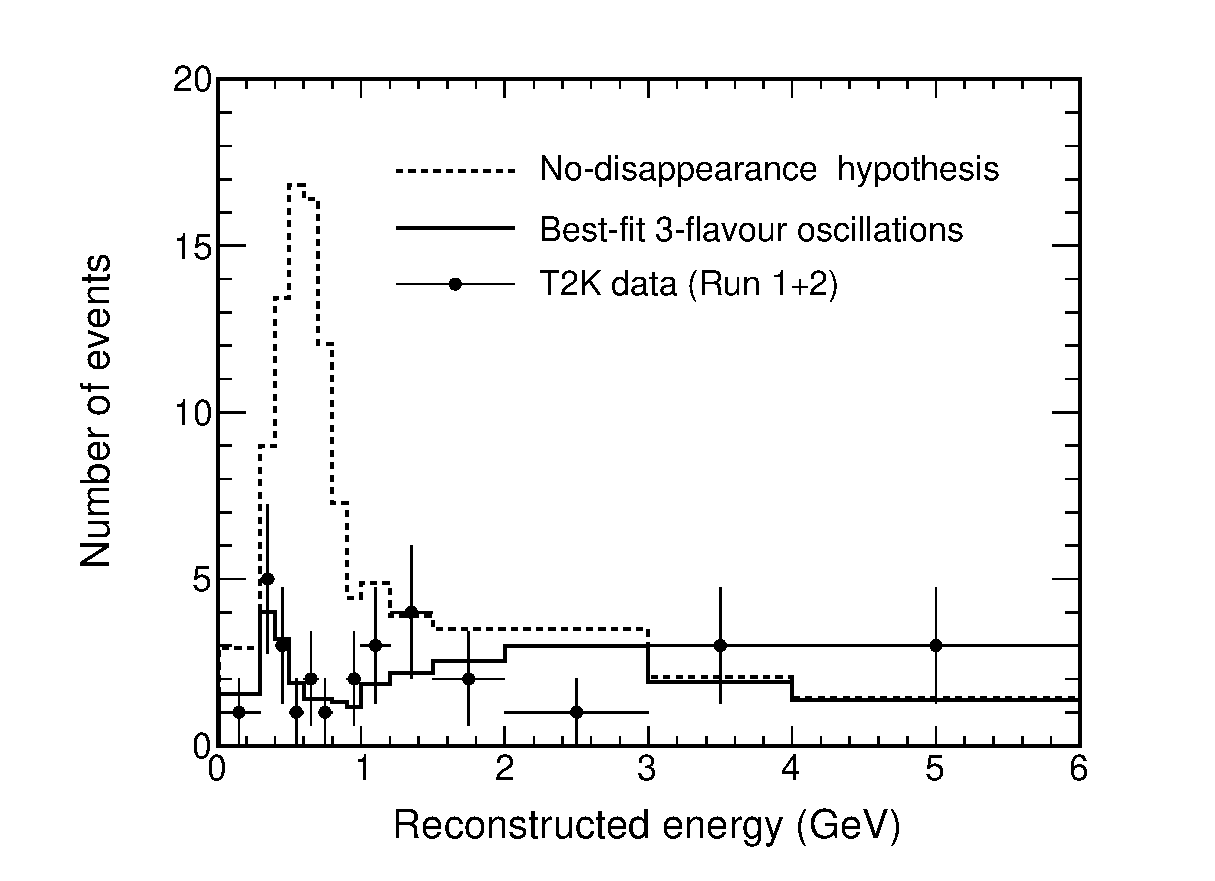
\includegraphics{./images/best_fit/SKErecoNullBestFitGenie.eps}}
\caption[Reconstructed energy spectrum of the 31 Run 1+2 data events compared with the expected spectra in Super-K without disappearance and
with best-fit 3-flavour oscillations (GENIE)]
{Reconstructed energy spectrum of the 31 Run 1+2 data events compared with the expected spectra in Super-K without disappearance and 
with best-fit 3-flavour oscillations (GENIE); the spectrum for best-fit oscillations uses $\sin^{2}(2 \theta_{12})$ = 0.87, $\sin^{2}(2 \theta_{13})$ = 0.1,
$\Delta m_{21}^{2}$ = 7.6 $\times 10^{-5}$ eV$^{2}$/c$^{4}$, $\delta_{CP}$ = 0 and Earth crust density = 2.6 g/cm$^{3}$. The atmospheric $\Delta m^{2}$ is input 
as $|\Delta m_{32}^{2}|$. A variable binning scheme is used here for the purpose of illustration only; the actual analysis used equal-sized 50 MeV bins.}
\label{bestfitdataexpectedgenie}
\end{center}
\end{figure}

\begin{figure}
\begin{center}
\resizebox{13cm}{!}{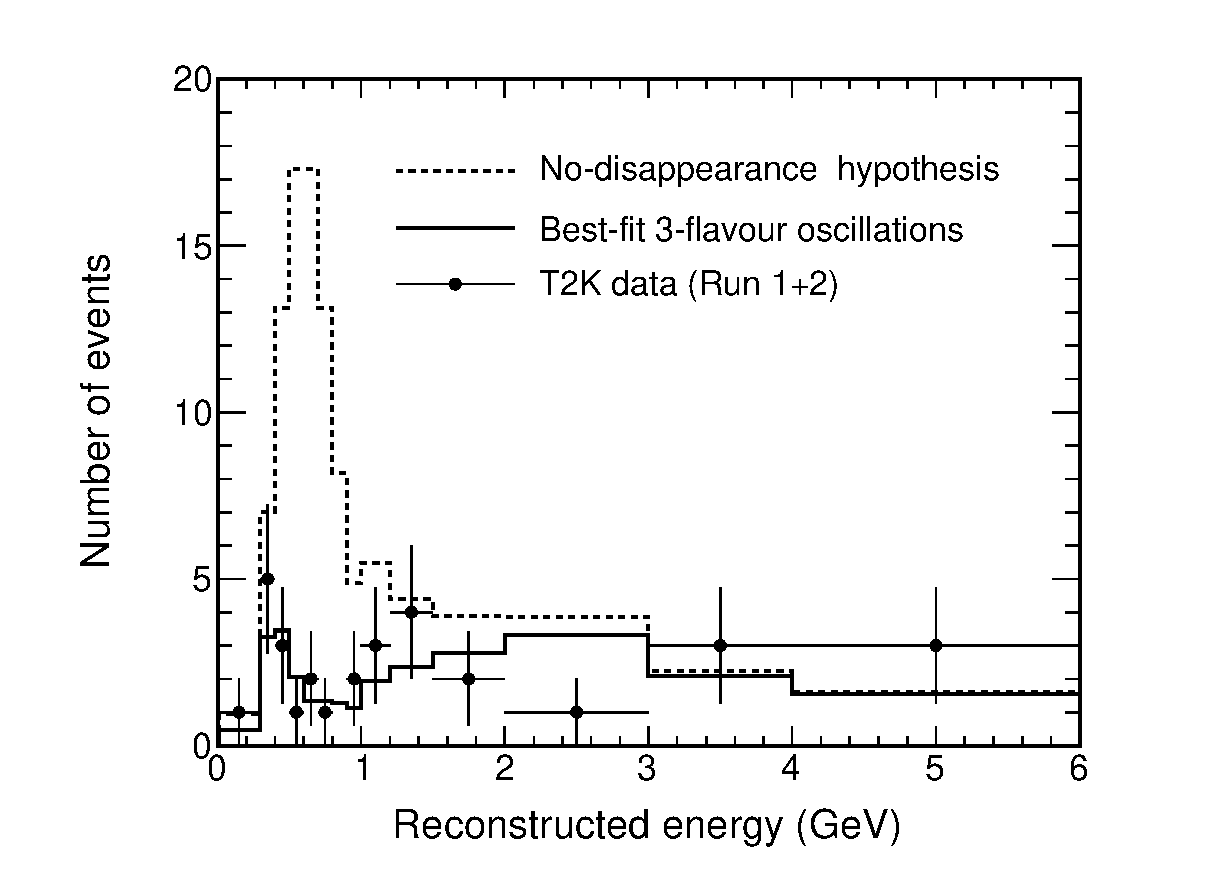
\includegraphics{./images/best_fit/SKErecoNullBestFitNeut.eps}}
\caption[Reconstructed energy spectrum of the 31 Run 1+2 data events compared with the expected spectra in Super-K without disappearance and
with best-fit 3-flavour oscillations (NEUT)]
{Reconstructed energy spectrum of the 31 Run 1+2 data events compared with the expected spectra in Super-K without disappearance and
with best-fit 3-flavour oscillations (NEUT); the spectrum for best-fit oscillations uses $\sin^{2}(2 \theta_{12})$ = 0.87, $\sin^{2}(2 \theta_{13})$ = 0.1,
$\Delta m_{21}^{2}$ = 7.6 $\times 10^{-5}$ eV$^{2}$/c$^{4}$, $\delta_{CP}$ = 0 and Earth crust density = 2.6 g/cm$^{3}$. The atmospheric $\Delta m^{2}$ is input
as $|\Delta m_{32}^{2}|$. A variable binning scheme is used here for the purpose of illustration only; the actual analysis used equal-sized 50 MeV bins.}
\label{bestfitdataexpectedneut}
\end{center}
\end{figure}

\begin{figure}
\begin{center}
\resizebox{13cm}{!}{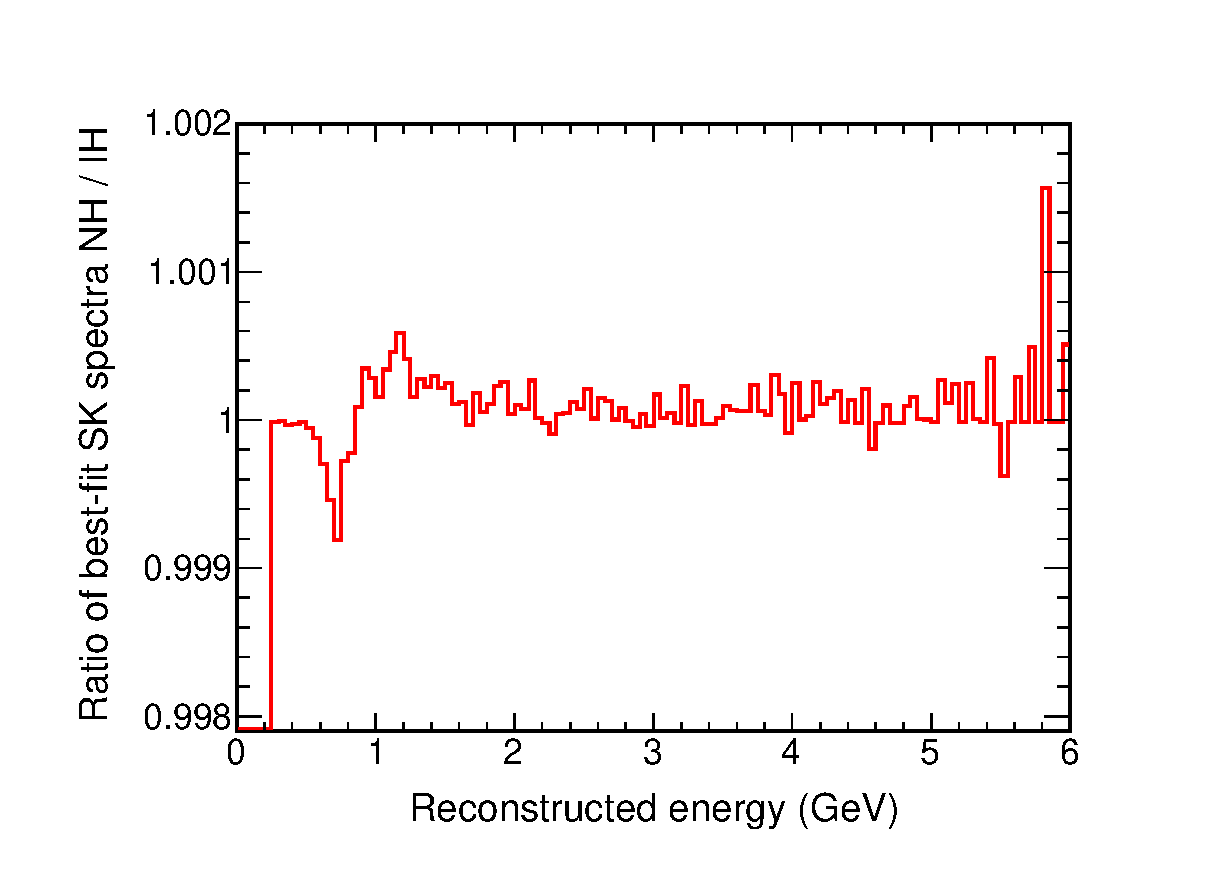
\includegraphics{./images/best_fit/BestFitRatioNormalInverted.eps}}
\caption[Ratio of best-fit 3-flavour reconstructed Super-K energy spectrum assuming the normal mass
hierarchy to that assuming the inverted mass hierarchy using NEUT]
{Ratio of best-fit 3-flavour reconstructed Super-K energy spectrum assuming the normal mass
hierarchy to that assuming the inverted mass hierarchy using NEUT; $\sin^{2}(2 \theta_{12})$ = 0.87, $\sin^{2}(2 \theta_{13})$ = 0.1,
$\Delta m_{21}^{2}$ = 7.6 $\times 10^{-5}$ eV$^{2}$/c$^{4}$, $\delta_{CP}$ = 0 and Earth crust density = 2.6 g/cm$^{3}$. The atmospheric 
$\Delta m^{2}$ is input as $|\Delta m_{32}^{2}|$.}
\label{rationormalinverted}
\end{center}
\end{figure}

\begin{figure}
\begin{center}
\resizebox{13cm}{!}{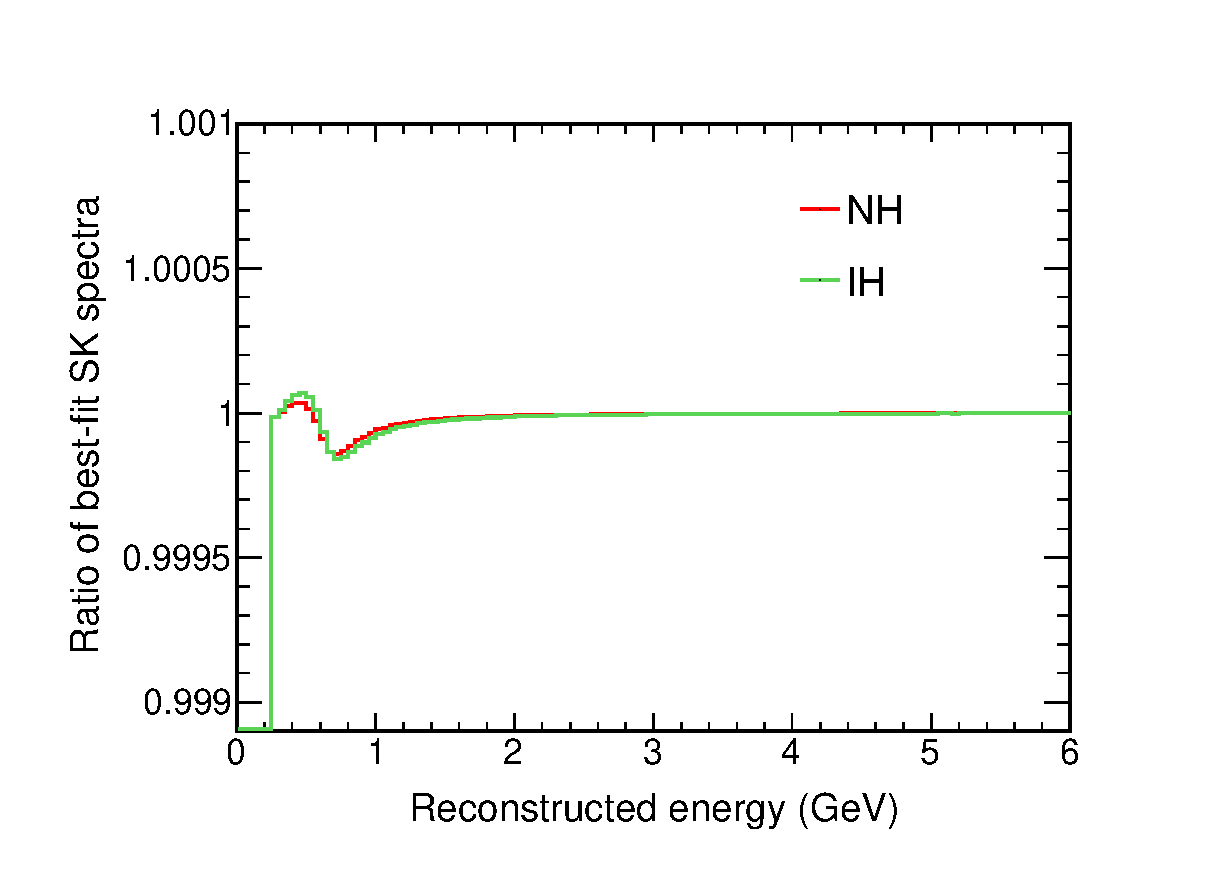
\includegraphics{./images/best_fit/BestFitRatioFogliLisi.eps}}
\caption[Ratio of best-fit 3-flavour reconstructed Super-K energy spectrum for the atmospheric $\Delta m^{2}$ input as $|\Delta m_{32}^{2}|$ to
the best-fit spectrum for the atmospheric $\Delta m^{2}$ input as $|\Delta m_{FL}^{2}|$ using NEUT]
{Ratio of best-fit 3-flavour reconstructed Super-K energy spectrum for the atmospheric $\Delta m^{2}$ input as $|\Delta m_{32}^{2}|$ to 
the best-fit spectrum for the atmospheric $\Delta m^{2}$ input as $|\Delta m_{FL}^{2}|$ = $|m_{3}^{2} - [(m_{2}^{2} + m_{1}^{2}) / 2]|$ using NEUT; 
$\sin^{2}(2 \theta_{12})$ = 0.87, $\sin^{2}(2 \theta_{13})$ = 0.1, $\Delta m_{21}^{2}$ = 7.6 $\times 10^{-5}$ eV$^{2}$/c$^{4}$, $\delta_{CP}$ = 0, Earth
crust density = 2.6 g/cm$^{3}$, NH = normal mass hierarchy, IH = inverted mass hierarchy.}
\label{ratiofoglilisi}
\end{center}
\end{figure}

The uncertainties in the best-fit values of $\sin^{2}(2 \theta_{23})$ and $|\Delta m_{32}^{2}|$ due to uncertainties in 
the values of the non-23 oscillation parameters were estimated by creating 50000 fake datasets for each mass 
hierarchy. These fake datasets did not include statistical fluctuations, and they were made using random input values of 
$\sin^{2}(2 \theta_{12})$, $\sin^{2}(2 \theta_{13})$ and $\Delta m_{21}^{2}$ drawn from Gaussian distributions with means 
equal to the nominal values and standard deviations equal to the 1$\sigma$ errors. The uncertainties in $\sin^{2}(2 \theta_{12})$ 
and $\Delta m_{21}^{2}$ are taken from KamLAND combined with solar experiments \cite{Kamland}, while those in 
$\sin^{2}(2 \theta_{13})$ are computed as a weighted average of measurements from Daya Bay \cite{DayaBay} and Reno \cite{Reno}. 
The input values of $\delta_{CP}$ were randomly drawn from a uniform distribution between -$\pi$ and +$\pi$. The input value of 
$\sin^{2}(2 \theta_{23})$ was fixed at 0.9 (to allow an estimate of both plus and minus uncertainties) and the input value of 
$|\Delta m_{32}^{2}|$ was fixed at 2.32 $\times$ 10$^{-3}$ eV$^{2}$/c$^{4}$. 

When fitting the fake datasets to obtain the best-fit points, the expected numbers of single $\mu$-like ring events in Super-K 
with oscillations were again calculated with fixed values of $\sin^{2}(2 \theta_{12})$, $\sin^{2}(2 \theta_{13})$, $\Delta m_{21}^{2}$ and $\delta_{CP}$, 
while $\sin^{2}(2 \theta_{23})$ and $|\Delta m_{32}^{2}|$ were allowed to vary in order to find their best-fit values. When all the non-23 
parameters were varied together, the standard deviations of the best-fit values of $\sin^{2}(2 \theta_{23})$ were 0.5\% (NH) and 0.4\% 
(IH), and those of the best-fit values of $|\Delta m_{32}^{2}|$ were 0.7\% (NH) and 0.4\% (IH). Additional fake datasets were made in which 
only one non-23 parameter was varied at a time, with the other parameters being fixed at their default values. The results are given in table 
\ref{bestfitnon23errors} which shows that the non-23 uncertainties in the best-fit points are almost entirely due to uncertainties in $\delta_{CP}$.
As a comparison, the uncertainties in the best-fit points due to the combined systematic uncertainties were considerably larger at 4.3\% (NH) 
and 4.9\% (IH) for $\sin^{2}(2 \theta_{23})$ and 4.8\% (NH) and 5.1\% (IH) for $|\Delta m_{32}^{2}|$. 

\begin{table}
\caption[Uncertainties in the best-fit values of $\sin^{2}(2 \theta_{23})$ and $|\Delta m_{32}^{2}|$ due to uncertainties in the non-23
oscillation parameters using NEUT]
{Uncertainties in the best-fit values of $\sin^{2}(2 \theta_{23})$ and $|\Delta m_{32}^{2}|$ due to uncertainties in the non-23 
oscillation parameters using NEUT. These are varied using random numbers drawn from Gaussian distributions with means equal to the nominal values and 
standard deviations equal to the 1$\sigma$ errors, except for $\delta_{CP}$ which is varied using a random number drawn from a uniform 
distribution between -$\pi$ and +$\pi$. When fixed these parameters have the values $\sin^{2}(2 \theta_{12})$ = 0.87, $\sin^{2}(2 \theta_{13})$ 
= 0.1, $\Delta m_{21}^{2}$ = 7.6 $\times$ 10$^{-5}$ eV$^{2}$/c$^{4}$, $\delta_{CP}$ = 0. The Earth crust density is taken to be 2.6 g/cm$^{3}$, and NH = 
normal mass hierarchy, IH = inverted mass hierarchy.}
\centering
\begin{tabular}{| c | c | c | c | c |}
\hline
Parameter & Uncertainty & Uncertainty & Uncertainty & Uncertainty \\
 & in $\sin^{2}(2 \theta_{23})$ & in $|\Delta m_{32}^{2}|$ & in $\sin^{2}(2 \theta_{23})$ & in $|\Delta m_{32}^{2}|$ \\
 & (NH) & (NH) & (IH) & (IH) \\
\hline
$\sin^{2}(2 \theta_{13})$ & 0.08\% & 0.2\% & 0.01\% & 0.05\%\\
\hline
$\delta_{CP}$ & 0.5\% & 0.6\% &  0.35\% & 0.4\%\\
\hline
$\sin^{2}(2 \theta_{12})$ & 0.004\% & 0.09\% & 0.007\% & 0.09\%\\
\hline
$\Delta m_{21}^{2}$ & 0.01\% & 0.04\% & 0.009\%  & 0.05\%\\
\hline
All non-23 parameters & 0.5\% & 0.7\% & 0.4\% & 0.4\%\\
\hline
All systematics & 4.3\% & 4.8\% & 4.9\% & 5.1\%\\
\hline
\end{tabular}
\label{bestfitnon23errors}
\end{table}

In order to show these uncertainties in the best-fit points graphically, they were also estimated by varying each non-23 parameter 
by $\pm$1$\sigma$ in a single toy experiment without statistical fluctuations. Once more the input value of $\sin^{2}(2 \theta_{23})$ was fixed 
at 0.9 and the input value of $|\Delta m_{32}^{2}|$ was fixed at 2.32 $\times$ 10$^{-3}$ eV$^{2}$/c$^{4}$. The results are shown in figure \ref{bestfitstarplot}, 
and the uncertainties in the best-fit points are again almost entirely due to uncertainties in $\delta_{CP}$.

\begin{figure}
\begin{center}
\resizebox{11cm}{!}{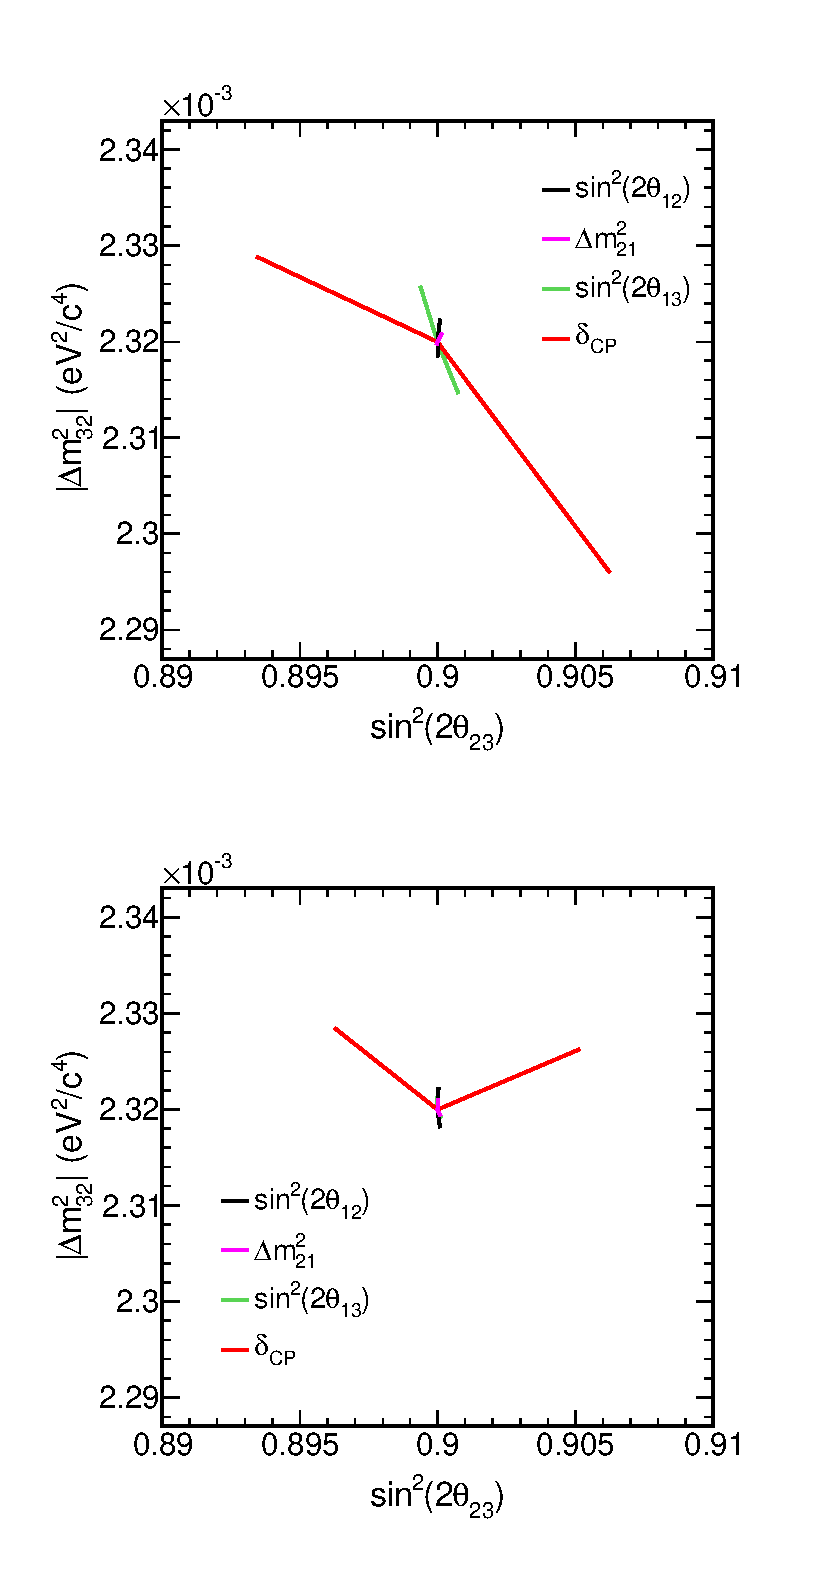
\includegraphics{./images/best_fit/BestFitStarPlot.eps}}
\caption[Uncertainties in the best-fit values of $\sin^{2}(2 \theta_{23})$ and $|\Delta m_{32}^{2}|$ due to uncertainties in the non-23
oscillation parameters for the normal mass hierarchy (top) and the inverted mass hierarchy (bottom) using NEUT]
{Uncertainties in the best-fit values of $\sin^{2}(2 \theta_{23})$ and $|\Delta m_{32}^{2}|$ due to uncertainties in the non-23 
oscillation parameters for the normal mass hierarchy (top) and the inverted mass hierarchy (bottom) using NEUT; uncertainties in $\delta_{CP}$ are shown 
for changes from 0 to +$\pi$/2 and -$\pi$/2.}
\label{bestfitstarplot}
\end{center}
\end{figure}

Since it is not curremtly possible to define a $\pm$1$\sigma$ error in $\delta_{CP}$, the effects of varying it on the best-fit values of 
$\sin^{2}(2 \theta_{23})$ and $|\Delta m_{32}^{2}|$ are plotted in figure \ref{bestfitstarplotdeltacp}. $\delta_{CP}$ can affect $|\Delta m_{32}^{2}|$ 
only (for example if it changes from 0.0 to $\pi$) or $\sin^{2}(2 \theta_{23})$ only (for example if it changes from 0.0 to $\frac{3\pi}{4}$) or 
both (for example if it changes from 0.0 to $\frac{\pi}{2}$).

\begin{figure}
\begin{center}
\resizebox{11cm}{!}{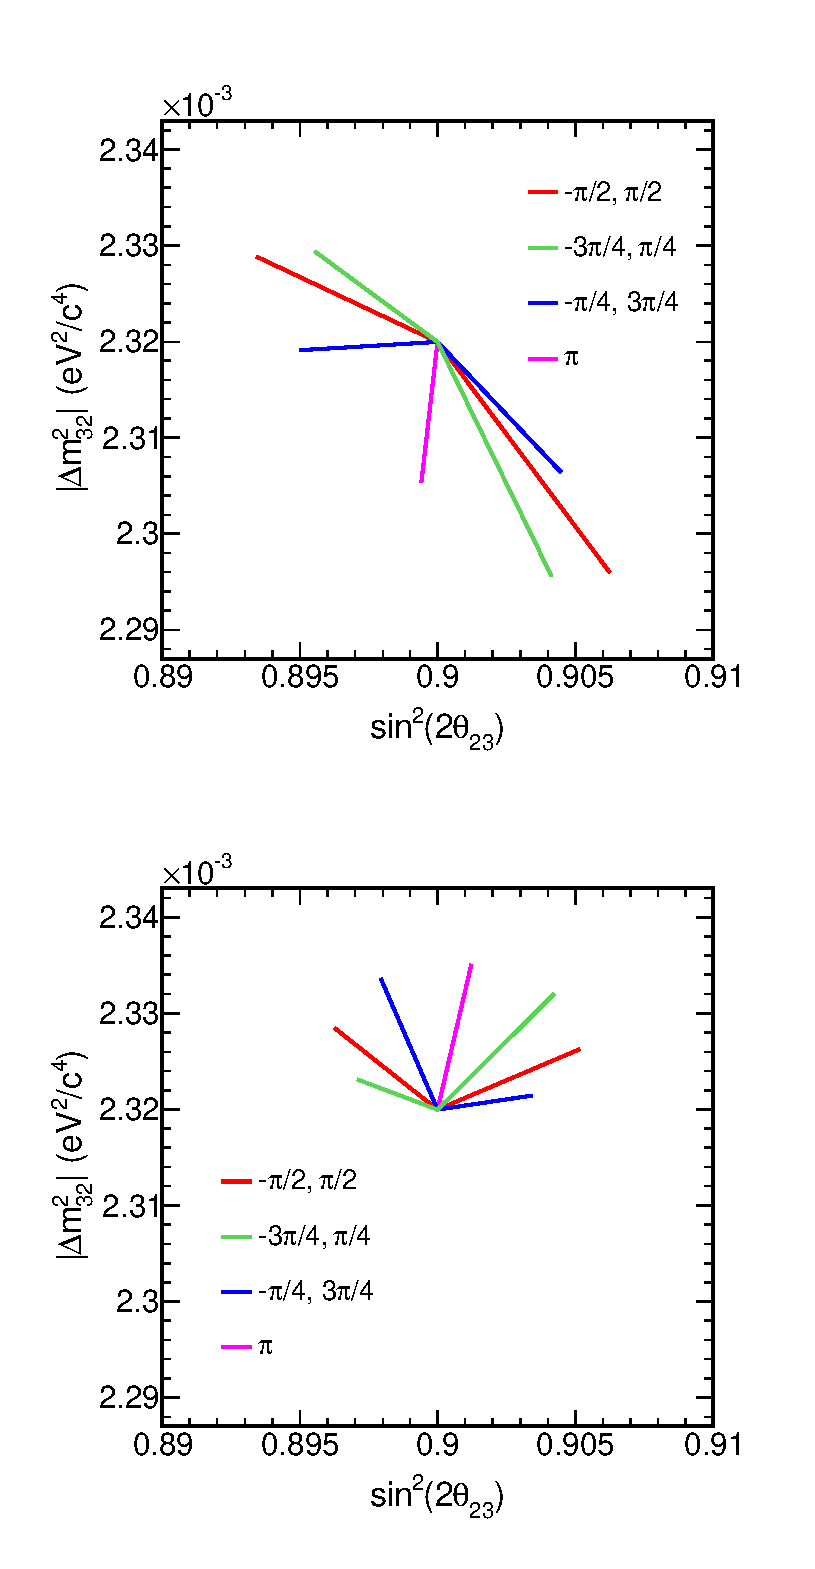
\includegraphics{./images/best_fit/BestFitStarPlotDeltaCP.eps}}
\caption{Uncertainties in the best-fit values of $\sin^{2}(2 \theta_{23})$ and $|\Delta m_{32}^{2}|$ due to uncertainties in $\delta_{CP}$ for the 
normal mass hierarchy (top) and the inverted mass hierarchy (bottom) using NEUT}
\label{bestfitstarplotdeltacp}
\end{center}
\end{figure}
